\documentclass[pdftex,12pt,a4paper]{article}
\usepackage[pdftex]{graphicx}
\usepackage{fancyhdr}
\usepackage{geometry}
\usepackage{draftcopy}
\usepackage{float}
\usepackage{amsmath}
\usepackage{algorithm2e}
\usepackage{color, colortbl}
\definecolor{Gray}{gray}{0.9}
\renewcommand{\thesection}{\arabic{section}.}
\renewcommand{\thesubsection}{\arabic{section}.\arabic{subsection} }
\renewcommand{\headrulewidth}{0pt}
\renewcommand{\footrulewidth}{0.5pt}
\pagestyle{fancy}
\fancyhead{}
\fancyfoot[LE,LO]{\footnotesize{
SE344, Chemistry and Our Environment
}
}

\title{\vspace{-15pt}Green Chemistry and Fate of Chemicals\\ SE344: Chemistry and Our Environment}
\author{Ankesh Kumar Singh (Y9090)}
\date{4th March, 2013}
\begin{document}
\maketitle
\begin{tabular}{p{370pt}}
\textbf{Keywords: }CO$_2$ absorption, chemical life cycle
\end{tabular}
\vspace{10pt}\\
\hrule
\vspace{10pt}
Industries produce a large amount of carbon dioxide by processes like fuel combustion and refining. Absorption of CO$_2$ is an important industrial problem as not many sinks are available. CO$_2$ being a greenhouse gas contributes to global warming and therefore, industries are bound by regulations as to how much CO$_2$ they can release into the atmosphere. At present, industries use the process of amine absorption in a scrubber to sequester CO$_2$.
\begin{center}
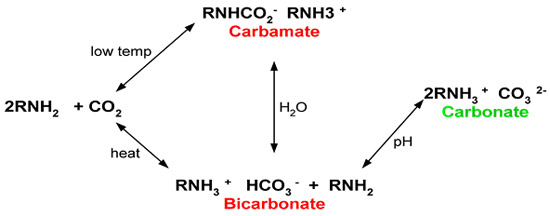
\includegraphics[scale=0.6]{4mari1.jpg}
\end{center}
Alkali metal bases can be used in a similar manner:
\vspace{5pt}\\
\begin{tabular}{rll}
2 NaOH + CO$_2$&$\rightarrow$& Na$_2$CO$_3$ + H$_2$O\\
Na$_2$CO$_3$ + Ca(OH)$_2$&$\rightarrow$&2 NaOH + CaCO$_3\downarrow$\\
CaCO$_3$&$\rightarrow $& CaO + CO$_2$
\end{tabular}\\
A process flow diagram is shown in Figure 1.
\begin{figure}[htb]
\centering
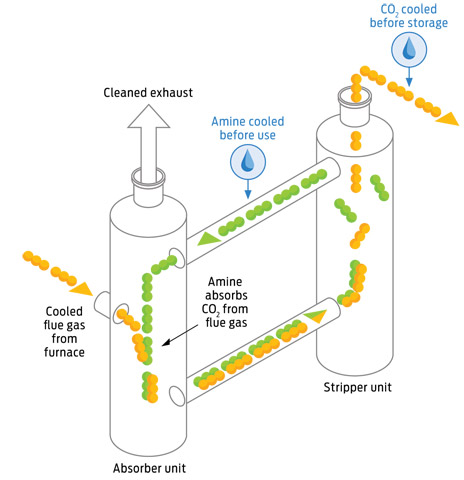
\includegraphics[scale=0.5]{4mari2.jpg}
\caption{CO$_2$ absorption unit}
\end{figure}
\\

In nature plants serve as an important sink for CO$_2$ by converting it into glucose, a useful form of food. Efforts have been made to find a suitable enzyme to make this conversion on an industrial scale. Many sea creatures convert carbon dioxide in the waters into calcium carbonate which is essentially chalk. Species such as clams, oysters and corals use it to make their shells and other bony parts. \\

When the team at Newcastle looked at the larvae of sea urchins they found that there were high concentrations of nickel on their external skeletons.
Working with extremely small nickel particles, the researchers found that when they added them to a solution of carbon dioxide in water, the nickel completely removed the CO2. \\

Predicting fate of chemicals in environment is important as any new process is centered around a new material. If harmful effects of CFCs on ozone layer could have been anticipated at the time they were introduced as refrigerants, alternatives like HFCs could have been introduced much earlier. However, making such predictions is very difficult.\\

There are complex compounds which are absorbed my micro organisms to form metabolites. They may be present in low to very low concentrations, even below detection limits. There are analytical difficulties in analyzing some compounds having unknown chemical properties and biological effects.\\

However, there is still hope for a reasonable analysis, due to previous experience of similar compounds like pesticides, priority pollutants. Large knowledge base of basic chemical principles expected to apply has been developed by previous risk assessments. Some chemicals are highly reactive with short half lives (NH$_3$, HCl, CO, SiCl$_4$) and others that are relatively inert (benzene, CFC). Several molecules that are normally inert may be induced to react. For example, when CFCs enter stratosphere, they dissociate due to UV radiations not present in the lower atmosphere.
\end{document}